\documentclass{article}
%\usepackage[utf8]{inputenc}
\usepackage{customPreamble}



\begin{document}
\begin{sloppypar}

    \begin{center}
    
        \Large{Paper Review For Gene2vec} \\
        \author{}{by Anurag Banerjee}\\
        
        \vspace{1em}
        \LARGE{\textbf{Gene2vec: distributed representation of genes \\ based on co-expression}\cite{gene2vec}} \\
    	\Large{\textit{Jingcheng Du et. al.}} \\
     
    \end{center}
	
    \begin{normalsize}
    
    	\begin{mybox}
    \textbf{Epigenomic} - Describes changes in regulation of gene activities that
        act independently of changes in gene sequences
\end{mybox}

\begin{mybox}
    \textbf{Decomposition} - Factorisation of a matrix or tensor into simpler terms
\end{mybox}

\begin{mybox}
    \textbf{Heterogeneous graph} - A graph that may contain more than one type of
        node and edge
\end{mybox}


		
		
		\section{Problem Description}
        This paper attempts to figure out, how to represent all human \textbf{gene}s as $n$-dimensional
		vectors, such that they also capture functional relatedness of the genes.
		These vectors are to be the \textit{distributed} representation of the genes,
		in line with word embeddings (as in Natural Language Processing or NLP).
                
        \section{Problem Relevance}
        A naive way to think of a \textbf{gene} is that, it is made up of multiple \textbf{transcript}s; where as all transcripts in the human \textbf{genome} have been identified, the \textbf{functional annotation}s of the gene is \textit{discrete}, \textit{categorical} and through \textit{manual efforts}.\\

		In NLP, a word's vector representation (neural embedding) depends on the co-occurrence of other words in the same sentence. Leveraging this idea, the authors have used \textbf{gene co-expression} as the basis of similarity for obtaining the \textit{\textbf{gene embeddings}}.\\

		Such gene embeddings may be used for multiple downstream tasks such as \textit{finding gene-gene interactions}, clustering the embeddings in some dimensional space to \textit{group genes into some functional group}, etc.
        
		\begin{sloppypar*}

    \noindent The authors have setup the downstream task as a link prediction problem,
    which roughly has $4$ stages:

    \begin{tabularx}{\textwidth}{XXXX}
        1. Build gene-disease graph & 2. Initial node features & 3. GCN & 4. Decoding
    \end{tabularx}

    \subsection{Building Heterogeneous gene-disease Graph}
        \begin{figure}
            \centering
            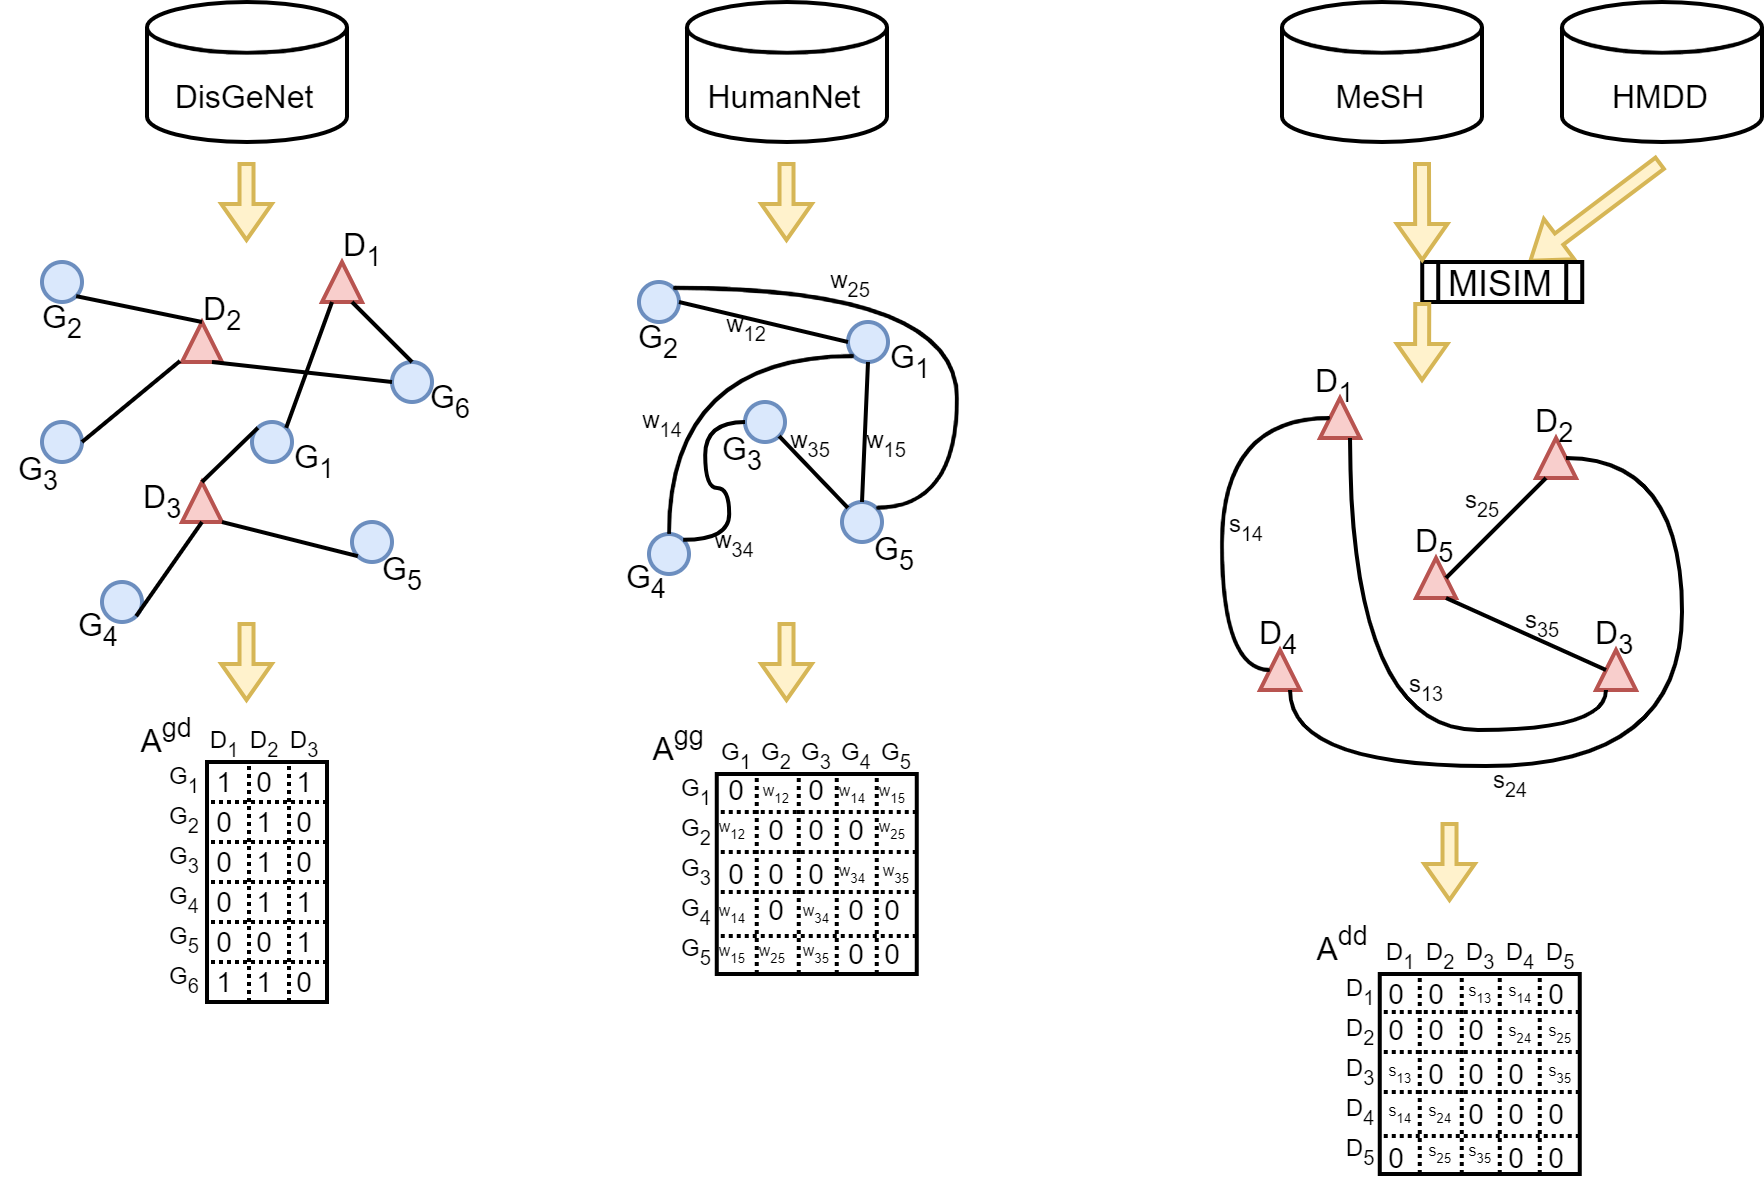
\includegraphics[scale=0.25]{EmbeddingsGCN_input.png}
            \caption{The adjacency matrices for the various edge types. The MISIM
                    \cite{DisDisEdge} method generates the scores for the disease-
                    disease edges. In the final heterogenous graph structure, the
                    vertex set is retained from the DisGeNet while the edge set is a
                    union of all the above three Adjacencies as per Eq. 1, 2, 3
                    in the paper.}
            \label{fig:heteroinput}
        \end{figure}

        \noindent As depicted in Figure \ref{fig:heteroinput} the primary data
        sources are \textbf{DisGeNet} for \textbf{gene-disease} linkages,
        \textbf{HumanNet} for \textbf{gene-gene} linkages and \textbf{MeSH $+$ 
        HMDD} for creating the \textbf{disease-disease} linkages from the DAG of
        MeSH. The DAG is used in a process called MISIM \cite{DisDisEdge} that
        generates scores that can be used for making the disease-only graph.\hfill\break

        \noindent Once we have the above information, the final heterogenous graph
        is constructed as $G = (V, E)$, where $V = V^{gd}$ and $E = E^{gd} \cup E^{gg} \cup E^{dd}$.
        The adjacency matrix is constructed as follows (\textit{Eq. 1, 2, 3 of the paper}):

        \begin{warning}
            \textbf{Disclaimer}: \textit{The equations that follow need reconsideration.
                I have modified a term.}
        \end{warning}

        \begin{equation}
            A = 
                \begin{bmatrix}
                    \tilde{A}^{gg} & A^{gd} \\
                    (A^{gd})^T & \tilde{A}^{dd} \\
                \end{bmatrix}
        \end{equation} 
        \noindent where,
        \begin{equation}
            \begin{aligned}
                \tilde{A}^{gg}_{ij} &= \phi^i A^{gg}_{ij} \\
                \phi^i &= \phi \frac{\sum_j A^{gd}_{ij}}{\sum_j A^{gg}_{ij}}
            \end{aligned}
        \end{equation}
        \begin{equation}
            \begin{aligned}
                \tilde{A}^{dd}_{ij} &= \phi^i A^{dd}_{ij} \\
                \phi^i &= \phi \frac{\sum_j A^{gd}_{ij}}{\sum_j A^{dd}_{ij}}
            \end{aligned}
        \end{equation}
        \noindent where, $\phi$ is normalized co-efficients (\textit{authors have
        not elaborated on the meaning}).

    \subsection{DeepWalk: generating initial node features}
        \textbf{RandomWalk -} After the graph is built, each node is assigned
        an index. For each node, DeepWalk selects $\lambda$ neighbours based on
        edge weights from the adjacency matrix $A$. These $\lambda$-length, index
        sequences form the input to word2vec.\hfill\break

        \textbf{Word2Vec -} The index sequences act as documents for a
        skip-gram version of the word2vec training model. With all the nodes (gene or
        disease) forming the vocabulary, the index sequences act as sentences. A
        one-hot vector is assigned to each node (based on its index). Then, for each
        node, context words are predicted for a fixed window size. The loss function
        (\textit{Eq. 4 in paper}) compares the prediction against the actual context
        words in the sequences (\textit{obtained from RandomWalk})\hfill\break

        \noindent The above two steps generate the initial feature vectors for each node in
        the heterogenous graph. The point to note is that these features only
        capture the \textbf{\textit{structural}} information of the graph.

    \begin{mybox}
        The GCN network by itself can not learn anything, unless there is a down-
        stream task. My understanding is that the decoder layer is essentially the
        downstream task for the GCN.
    \end{mybox}
    
    \subsection{Node embeddings via Graph Convolution Network}
        At this point, we have a graph (heterogeneous) and initial node-features.
        Kipf's GCN \cite{kipfGCN} has a good application in this scenario to learn
        even better connectivity embeddings for the nodes. Through message passing
        via the \textit{symmetric degree normalized} adjacency matrix, each node
        eventually learns about all other nodes in the graph (over multiple iterations,
        all hop information is spread). All that is needed is a downstream task.

        \begin{equation}
            \mathit{embeddings} = 
                \sigma (\tilde{D}^{\frac{1}{2}} \tilde{A} \tilde{D}^{-\frac{1}{2}} X \Theta)
        \end{equation}

    \subsection{Decoding novel gene-disease pairs}
        For the downstream task, the authors concatenate embeddings of a gene and
        a disease  and let a $3$-layer FFNN predict the probabilities for a valid
        association or an invalid association (essentially a binary classification).
        For this, the set of positive connections and negative connections are drawn
        from the graph $G$. The loss function is a combination of \textbf{negative log-likelihood}
        and a novel \textbf{cluster loss} (\textit{which looks at approximate clusters based
        on cosine similarity of the embedding vectors}). The clusters in question
        are approximate in the sense that a node is assigned to a cluster based
        on a \textit{cluster centre} calculated within a distance threshold.\hfill\break
    
    \noindent \textbf{Gene Prioritization -} It essentially means assigning ranks
    to genes based on weighted associations to a particular disease. The first step
    is to list all genes with \textbf{valid} associations (from section $4.4$) for
    some disease. Next, filter the list based on a threshold on the association
    probability score. The final step is to sort the filtered gene list according
    to their DeepWalk probability score. The result is the final output (
    \textit{Table III in the paper is an example}).

    % \begin{markdown}
    % \end{markdown}
    % \begin{figure}
    %     \centering
    %     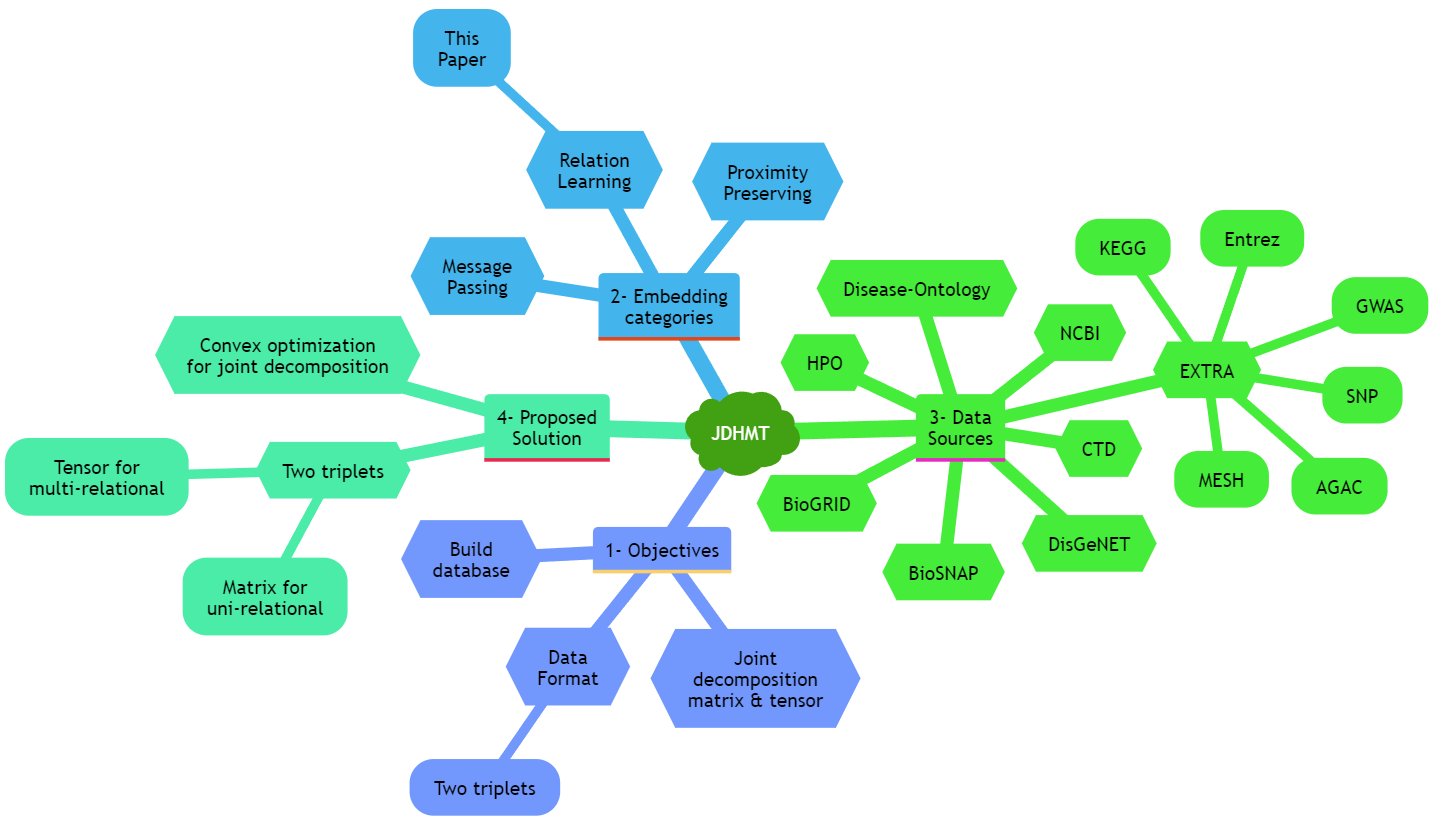
\includegraphics[width=170mm,scale=1]{mindmap.png}
    %     \caption{Mindmap}
    %     \label{fig:mindmap}
    % \end{figure}

\end{sloppypar*}
	   	
	   	\section{Positive Points}
	   	\begin{itemize}
	   	    \item The paper utilizes concepts present in established NLP pipelines to create learned gene embeddings that are shown to be useful in downstream ML tasks.
	   	\end{itemize}
	   	
	   	\section{Negative Points}
	   	\begin{itemize}
			\item The description of the embedding generation could have been better
			\item The data sources may not reflect updated knowledge in the domain
	   	\end{itemize}
	   	
	   	\section{Questions}
	   	\begin{enumerate}
	   	    \item The use of micro-array based co-expression info could be outdated - will that affect the embedding generation?
			\item The actual steps in utilizing the data sources for creation of input data is not clear. What are the steps?
			\item The exact description of the loss function is slightly dubious. Can it be improved?
	   	\end{enumerate}

    \end{normalsize}
    
    \bibliographystyle{ieeetr}
    \bibliography{reference}
  
\end{sloppypar}
\end{document}